\documentclass[10pt]{article}
\usepackage[export]{adjustbox}
\usepackage{amsmath}
\usepackage[makeroom]{cancel}
\usepackage{enumitem}
\usepackage{graphicx}
%Load mhchem using some package options
\usepackage[version=4]{mhchem}
\usepackage{multicol}
\usepackage{siunitx}

\title{
    Problem Set \#8
    \\  \small
    CHEM101A: General College Chemistry
    }
\author{Donald Aingworth IV}
\date{October 10, 2025}

\newcommand{\E}[1]{\times 10^{#1}}
\newcommand{\U}[1]{\underline{#1}}

\begin{document}
    \DeclareSIUnit{\atm}{atm}
    \DeclareSIUnit{\molarity}{M}
    \DeclareSIUnit{\M}{M}
    \DeclareSIUnit{\torr}{torr}

    \maketitle

    \setcounter{section}{22}

    \pagebreak
    \section{Topic D Problem 23}
        Using the enthalpies of formation in \textbf{T1: Standard Thermodynamic Quantities} of your online textbook, calculate the amount of heat that will be released when 5.00 g of solid \ce{NaNO3} reacts with excess graphite in an open container. 
        The chemical equation for this reaction is:
        \begin{center}
            \ce{4 NaNO3(s) + 5 C(s, graphite) -> 2 Na2O(s) + 2 N2(g) + 5 CO2(g)}
        \end{center}

        \subsection{Solution}
            We can divide this reaction into two separate parts: the decomposition of the \ce{NaNO3} and the recomposition of \ce{Na2O} and \ce{CO2}.
            \begin{gather}
                \ce{NaNO3(s) -> Na(s) + \frac{1}{2}N2(g) + \frac{3}{2}O2(g), \Delta H = 467.9\,\unit{\kilo\joule/\mole}}\\
                \ce{2Na(s) + \frac{1}{2}O2(g) -> Na2O(s), \Delta H = -414.2\,\unit{\kilo\joule/\mole}}\\
                \ce{C(s, graphite) + O2(g) -> CO2(g), \Delta H = -393.5\,\unit{\kilo\joule/\mole}}
            \end{gather}

            Multiply the first by four, the second by two, and the third by five. 
            \begin{gather}
                \ce{4NaNO3(s) -> 4Na(s) + 2N2(g) + 6O2(g), \Delta H = 1871.6\,\unit{\kilo\joule/\mole}}\\
                \ce{4Na(s) + O2(g) -> 2Na2O(s), \Delta H = -828.4\,\unit{\kilo\joule/\mole}}\\
                \ce{5C(s, graphite) + 5O2(g) -> 5CO2(g), \Delta H = -1967.5\,\unit{\kilo\joule/\mole}}
            \end{gather}

            Add all of these together. for the sake of simplification, I will denote the cancelations out early.
            \begin{gather}
                \ce{4NaNO3(s) -> \cancel{4Na(s)} + 2N2(g) + \cancel{6O_2(g)}, \Delta H = 1871.6\,\unit{\kilo\joule/\mole}}\\
                \ce{\cancel{4Na(s)} + \cancel{O_2(g)} -> 2Na2O(s), \Delta H = -828.4\,\unit{\kilo\joule/\mole}}\\
                \ce{5C(s, graphite) + \cancel{5O_2(g)} -> 5CO2(g), \Delta H = -1967.5\,\unit{\kilo\joule/\mole}}\\
                \ce{4 NaNO3(s) + 5 C(s, graphite) -> 2 Na2O(s) + 2 N2(g) + 5 CO2(g)}
            \end{gather}

            The total enthalpy would be the sum of all enthalpies.
            \begin{equation}
                \Delta H = \Delta H_1 + \Delta H_2 + \Delta H_3 = -924.3\,\unit{\kilo\joule/\mole}
            \end{equation}

            Now convert the 5 grams of solid \ce{NaNO3} to moles. 
            \begin{gather}
                MM(\ce{NaNO3})  =   22.99 + 14.01 + 48.00
                    =   85.00\,\unit{\gram/\mole}\\
                n(\ce{NaNO3})   =   \frac{m}{MM}
                    =   \frac{5.00\,\unit{gram}}{85.00\,\unit{\gram/\mole}}
                    =   0.0588\,\unit{\mole}
            \end{gather}

            Multiply this by the enthalpy to find the heat.
            \begin{align}
                Q   =   \frac{n * \Delta H}{n_{\ce{NaNO3}}}
                    =   \frac{0.0588\,\unit{\mole} * (-924.3\,\unit{\kilo\joule/\mole})}{4}
                    =   -13.6\,\unit{\kilo\joule}
            \end{align}

            Since it's negative, that means it releases \boxed{13.6\,\unit{\kilo\joule}}. 

    \pagebreak
    \section{Topic D Problem 24}
        Pyrrole (\ce{C4H5N}) is a liquid that reacts with oxygen as follows:
        \begin{center}
            \ce{4 C4H5N(l) + 21 O2(g) -> 16 CO2(g) + 10 H2O(l) + 2 N2(g), \Delta H = -9407 kJ}
        \end{center} 
        Using this information and the enthalpies of formation in \textbf{T1: Standard Thermodynamic Quantities} of your online textbook, calculate the enthalpy of formation ($\rm \Delta H_f^{\circ}$) of \ce{C4H5N(l)}.

        \subsection{Solution}
            \begin{center}
                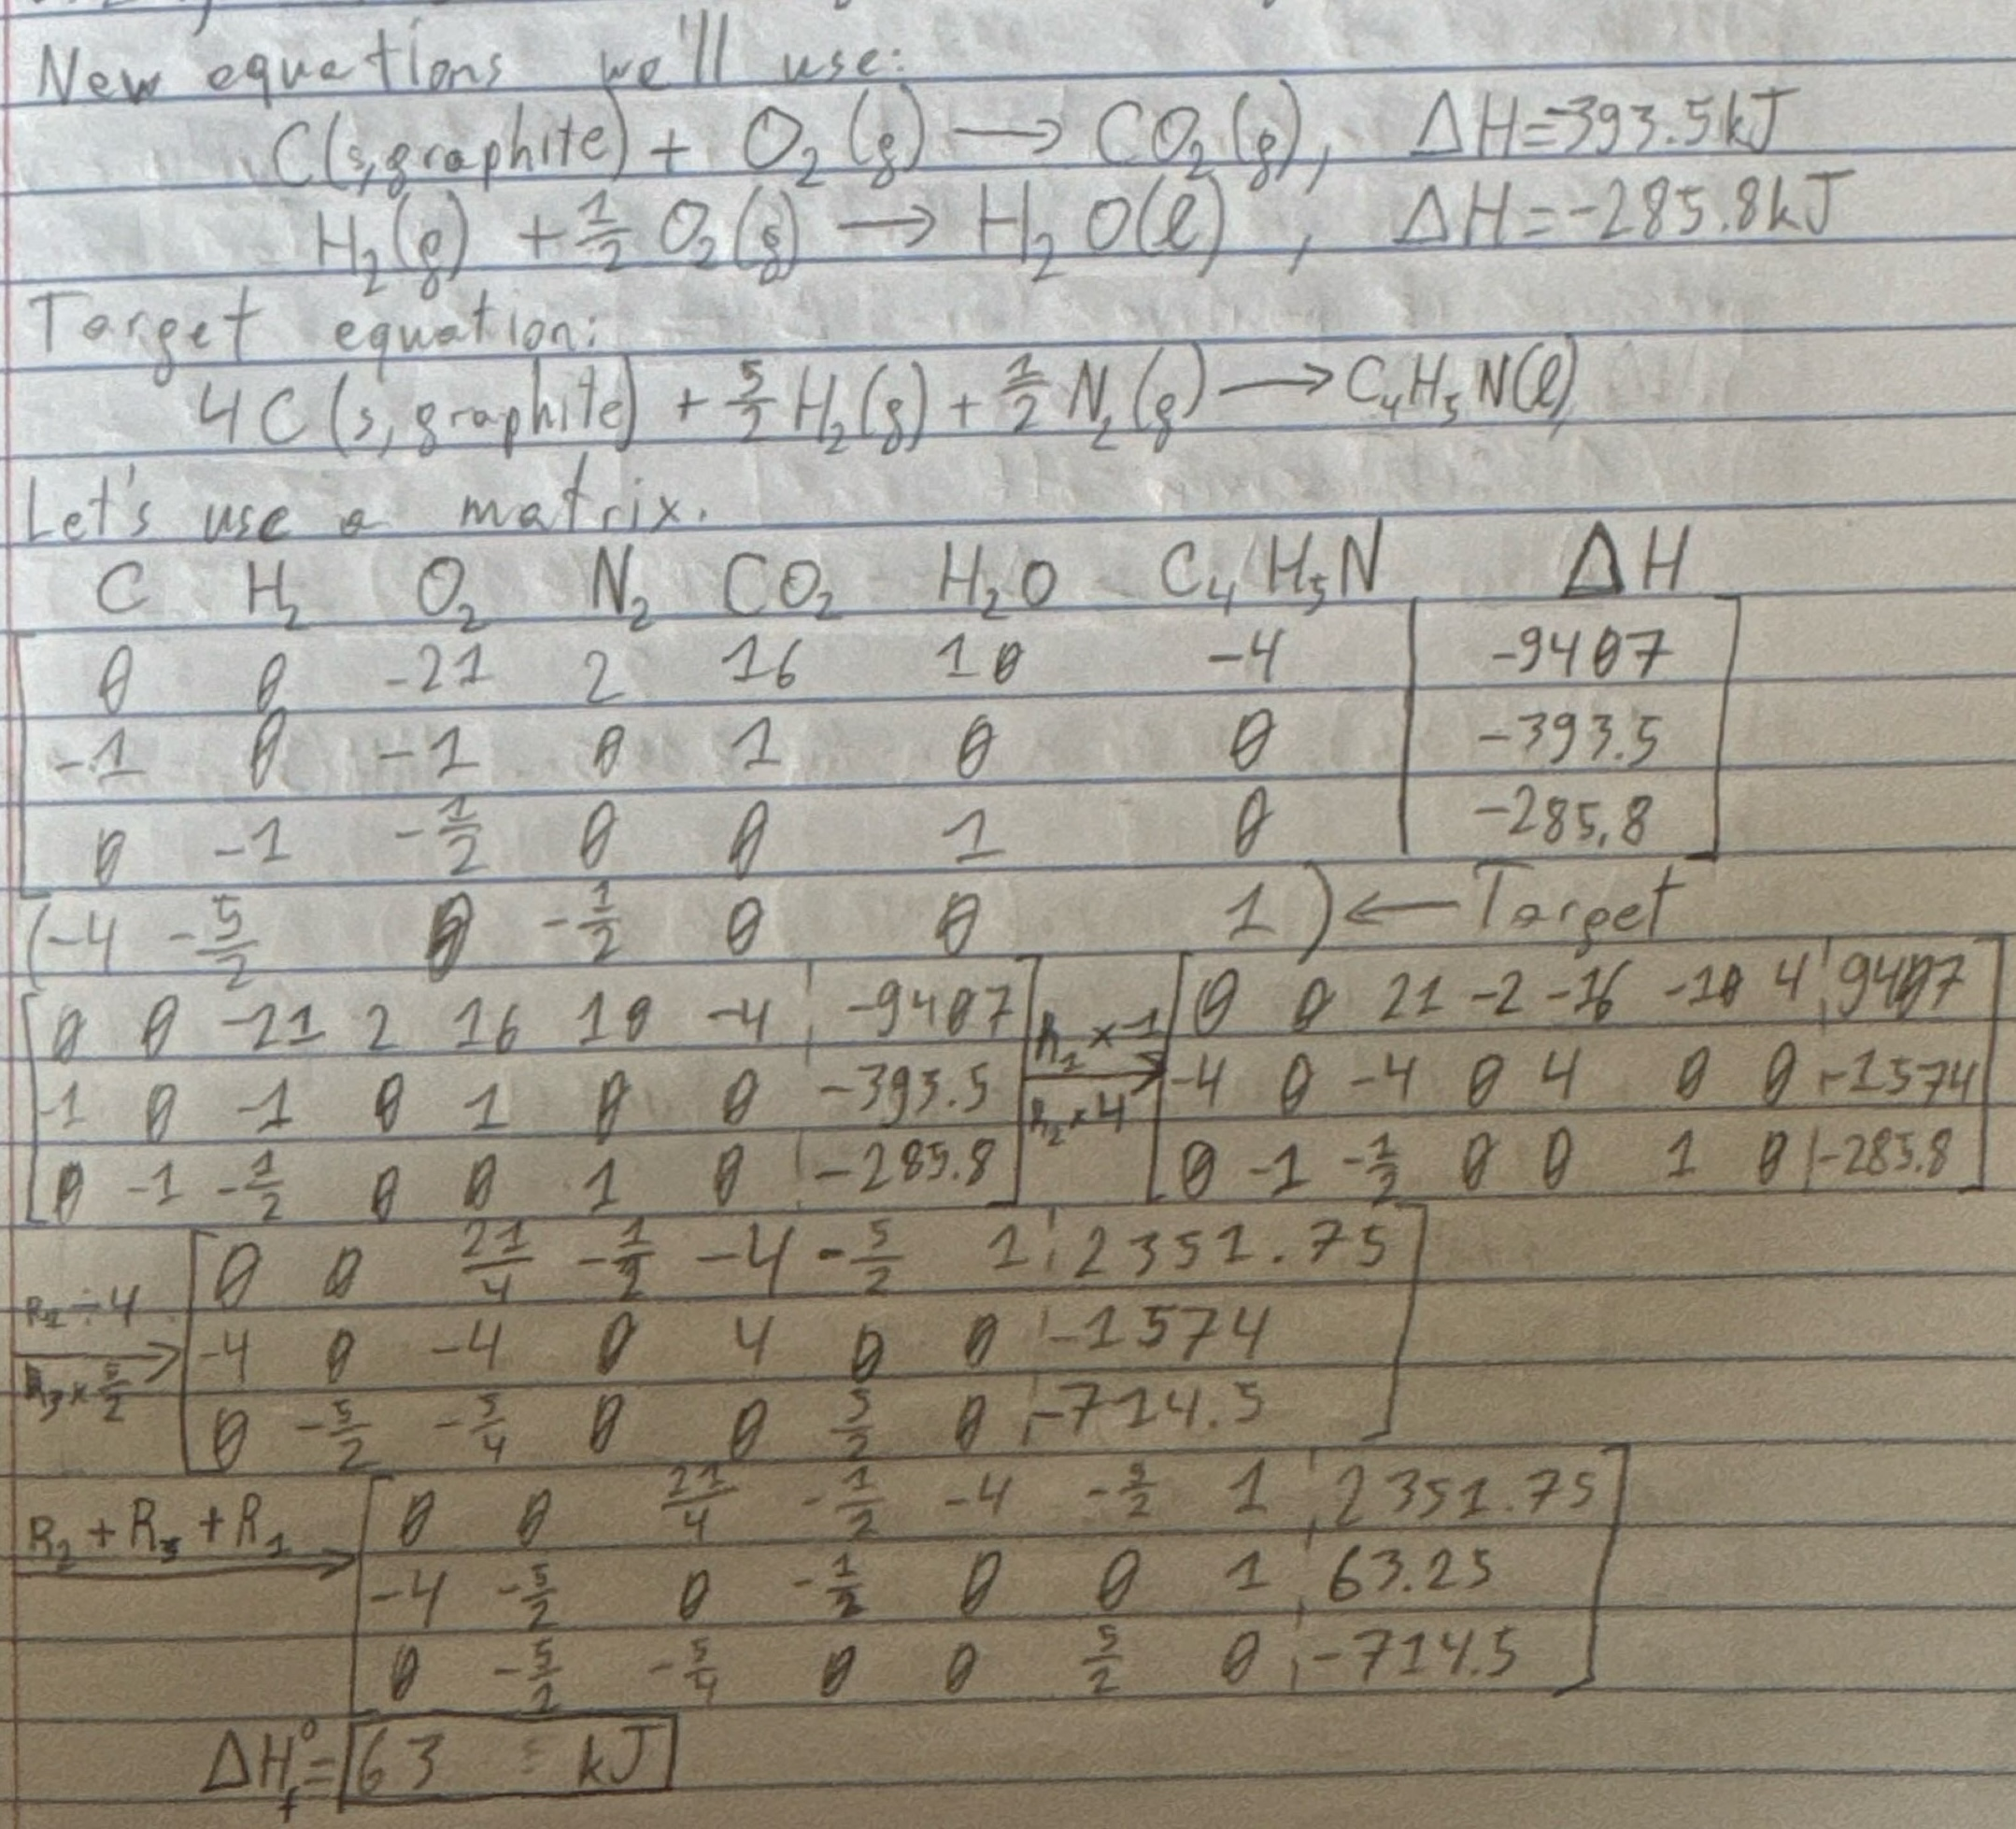
\includegraphics[width=\textwidth]{Answers Images/D24.jpg}
            \end{center}



    \pagebreak
    \section{Topic D Problem 25}
        For the reaction \ce{4 K(s) + O2(g) -> 2 K2O(s), \Delta H = -722 kJ}. 
        Using this information, calculate $\Delta$H for each of the following three reactions.
        \begin{enumerate}[label=\alph*)]
            \item   \ce{12 K(s) + 3 O2(g) -> 6 K2O(s)}
            \item   \ce{K(s) + 1/4 O2(g) -> 1/2 K2O(s)}
            \item   \ce{12 K2O(s) -> 24 K(s) + 6 O2(g)}
        \end{enumerate}

        \subsection{Solution}
            \begin{center}
                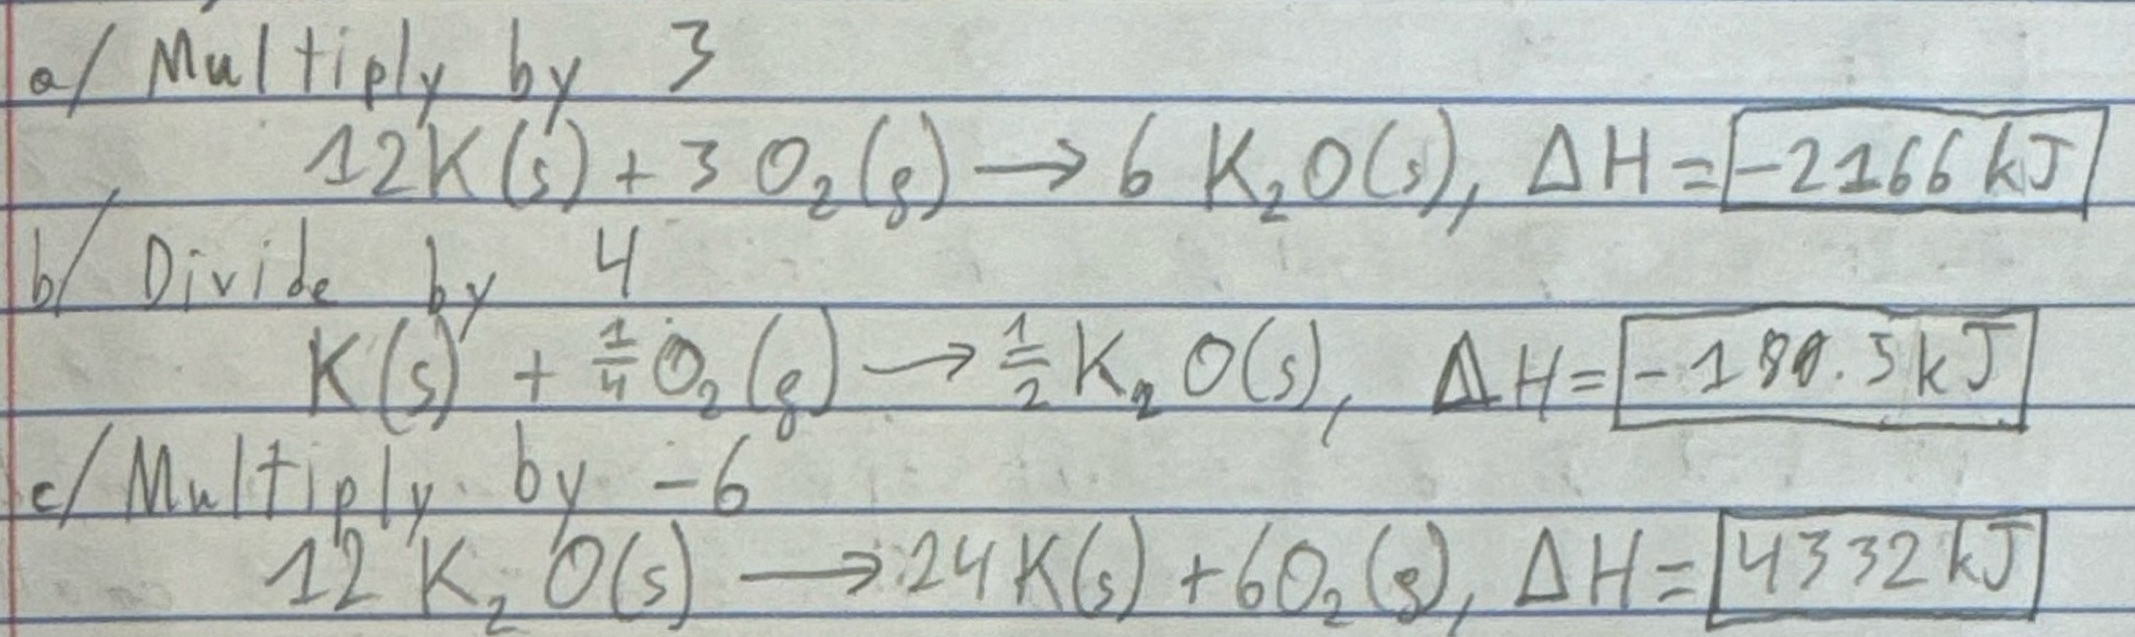
\includegraphics[width=\textwidth]{Answers Images/D25.jpg}
            \end{center}



    \pagebreak
    \section{Topic D Problem 26}
        Given the following chemical reactions and $\Delta$H values:
        \begin{align*}
            &\ce{3 Ag+(aq) + PO4^3-(aq) -> Ag3PO4(s)}   &\rm \Delta H = -32.7\,\unit{\kilo\joule}\\
            &\ce{Ag+(aq) + Cl-(aq) -> AgCl (s)}         &\rm \Delta H = -65.5\,\unit{\kilo\joule}
        \end{align*}
        Calculate $\Delta$H for the chemical reaction below:
        \begin{center}
            \ce{Ag3PO4(s) + 3 Cl- -> 3 AgCl(s) + PO4^3-(aq)}
        \end{center}

        \subsection{Solution}
            \begin{center}
                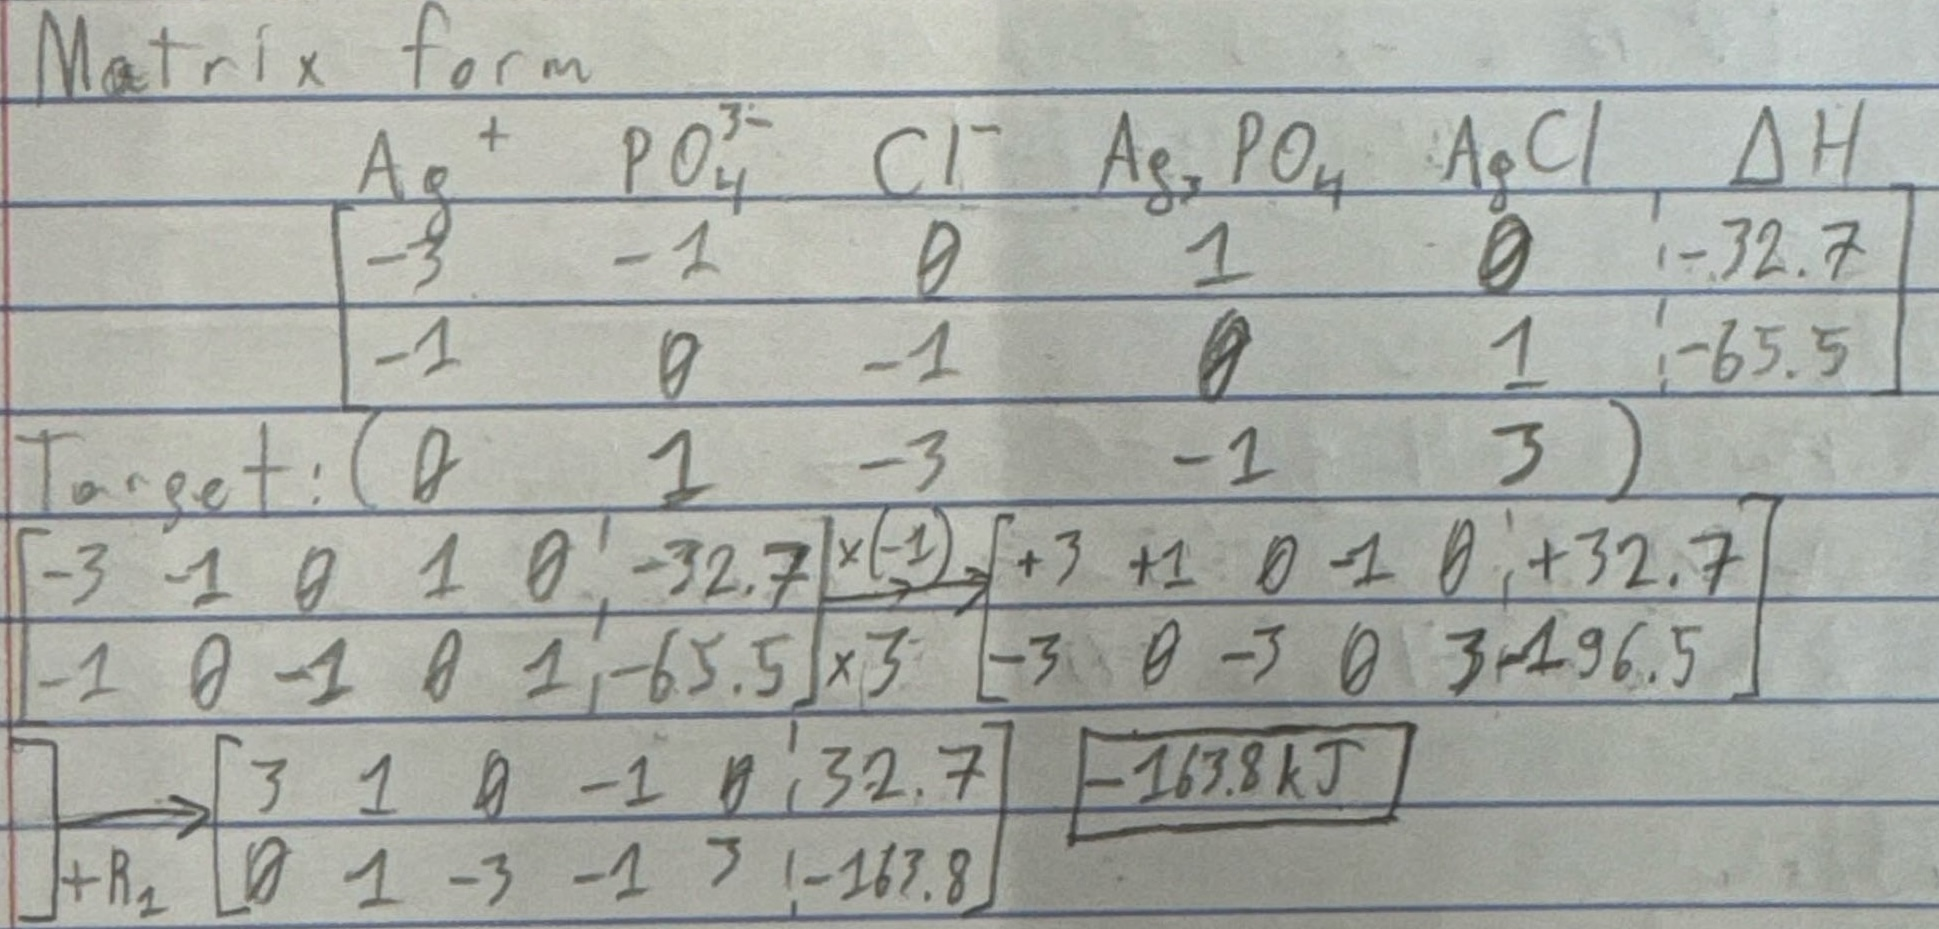
\includegraphics[width=\textwidth]{Answers Images/D26.jpg}
            \end{center}



    \pagebreak
    \section{Topic D Problem 27}
        Given the following chemical reactions and $\Delta$H values:
        \begin{align*}
            &\ce{As2O5(s) + 3 H2O(l) -> 2 H3AsO4(s)}            &\rm \Delta H = -30.2\,\unit{\kilo\joule}\\
            &\ce{H3AsO4(s) + 3 KOH(s) -> K3AsO4(s) + 3 H2O(l)}  &\rm \Delta H = -31.6\,\unit{\kilo\joule}\\
            &\ce{2 KOH(s) -> K2O(s) + H2O(l)}                   &\rm \Delta H = 202.0\,\unit{\kilo\joule}
        \end{align*}
        Calculate $\Delta$H for the chemical reaction below:
        \begin{center}
            \ce{As2O5(s) + 3 K2O(s) -> 2 K3AsO4(s)}
        \end{center}

        \subsection{Solution}
            \begin{center}
                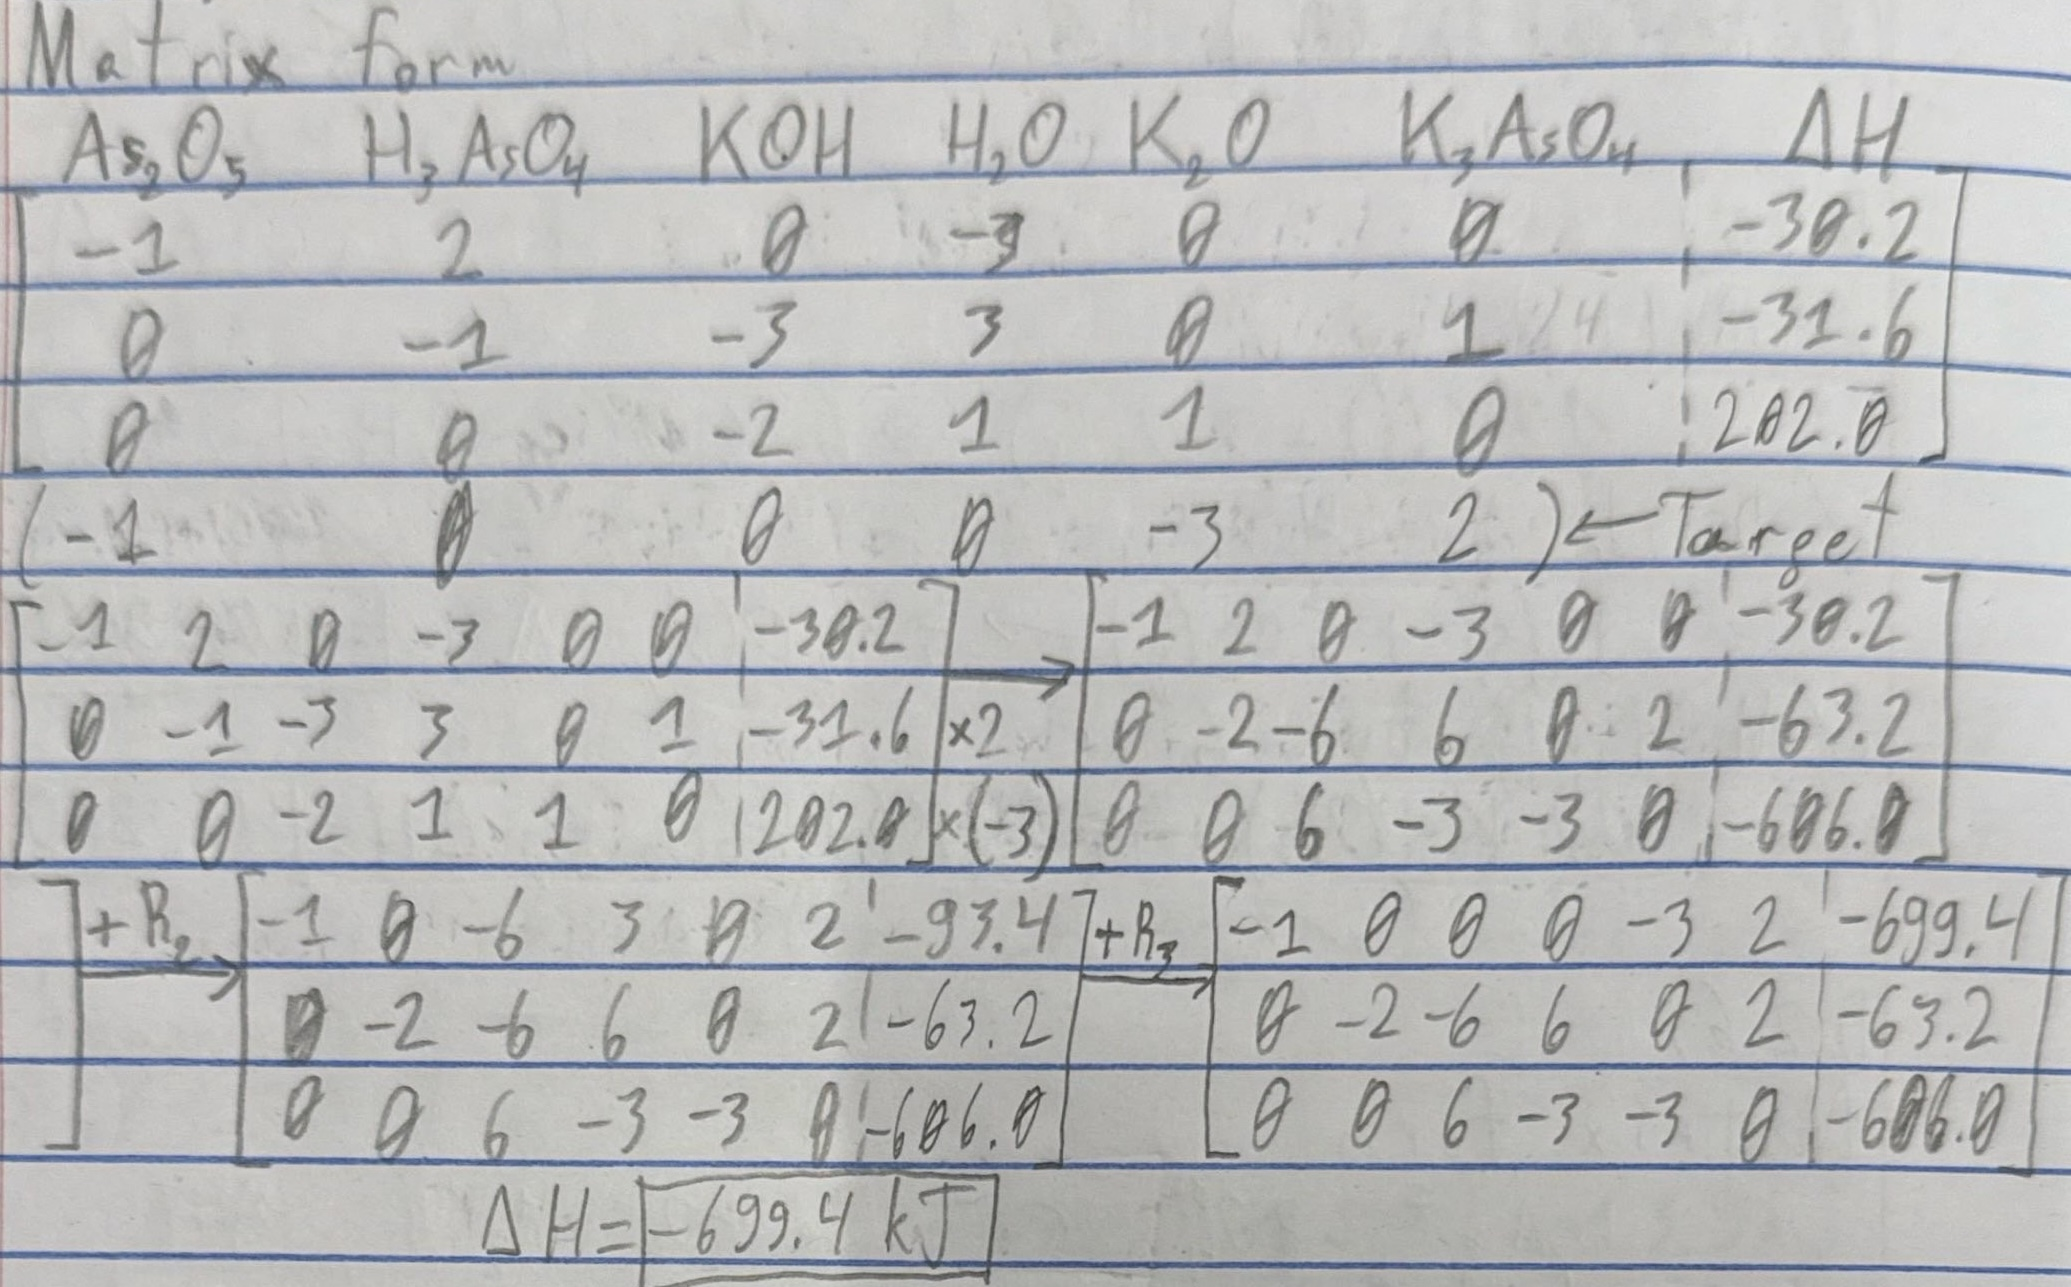
\includegraphics[width=\textwidth]{Answers Images/D27.jpg}
            \end{center}


    \pagebreak
    \section{Topic D Problem 28}
        The enthalpy of fusion ($\rm \Delta H_f^{\circ}$) of solid \ce{AgNO3} is -124 kJ/mol.
        \begin{enumerate}[label=\alph*)]
            \item   Based on this information, write a balanced chemical equation for which $\Delta$H = -124 kJ. Include the state of each substance in your equation.
            \item   Write a balanced chemical equation for which $\Delta$H = 124 kJ.
            \item   Write a balanced chemical equation for which $\Delta$H = -62 kJ. Hint: 124 = 2 \texttimes 62.
        \end{enumerate}

        \subsection{Solution}
            \begin{center}
                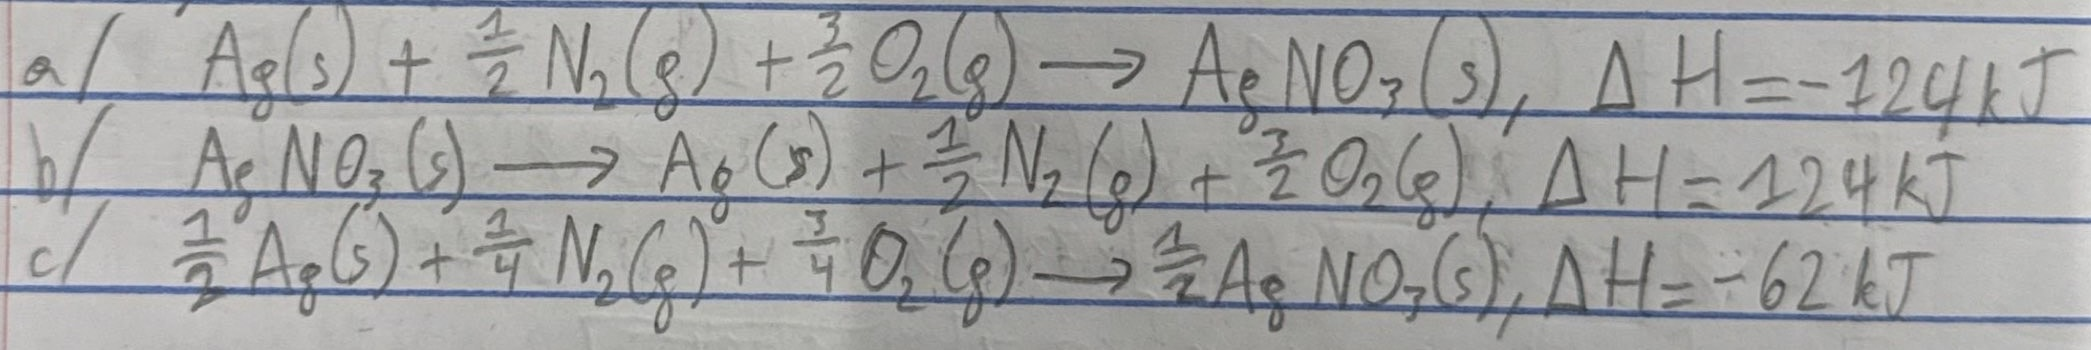
\includegraphics[width=\textwidth]{Answers Images/D28.jpg}
            \end{center}



    \pagebreak
    \section{Topic D Problem 29}
        The enthalpy of formation of solid \ce{AgBr} is -100.4 kJ. 
        Based on this information, can you calculate $\Delta$H for the reaction \ce{Ag+(aq) + Br-(aq) -> AgBr(s)}? 
        Explain why or why not.

        \subsection{Solution}
            \begin{center}
                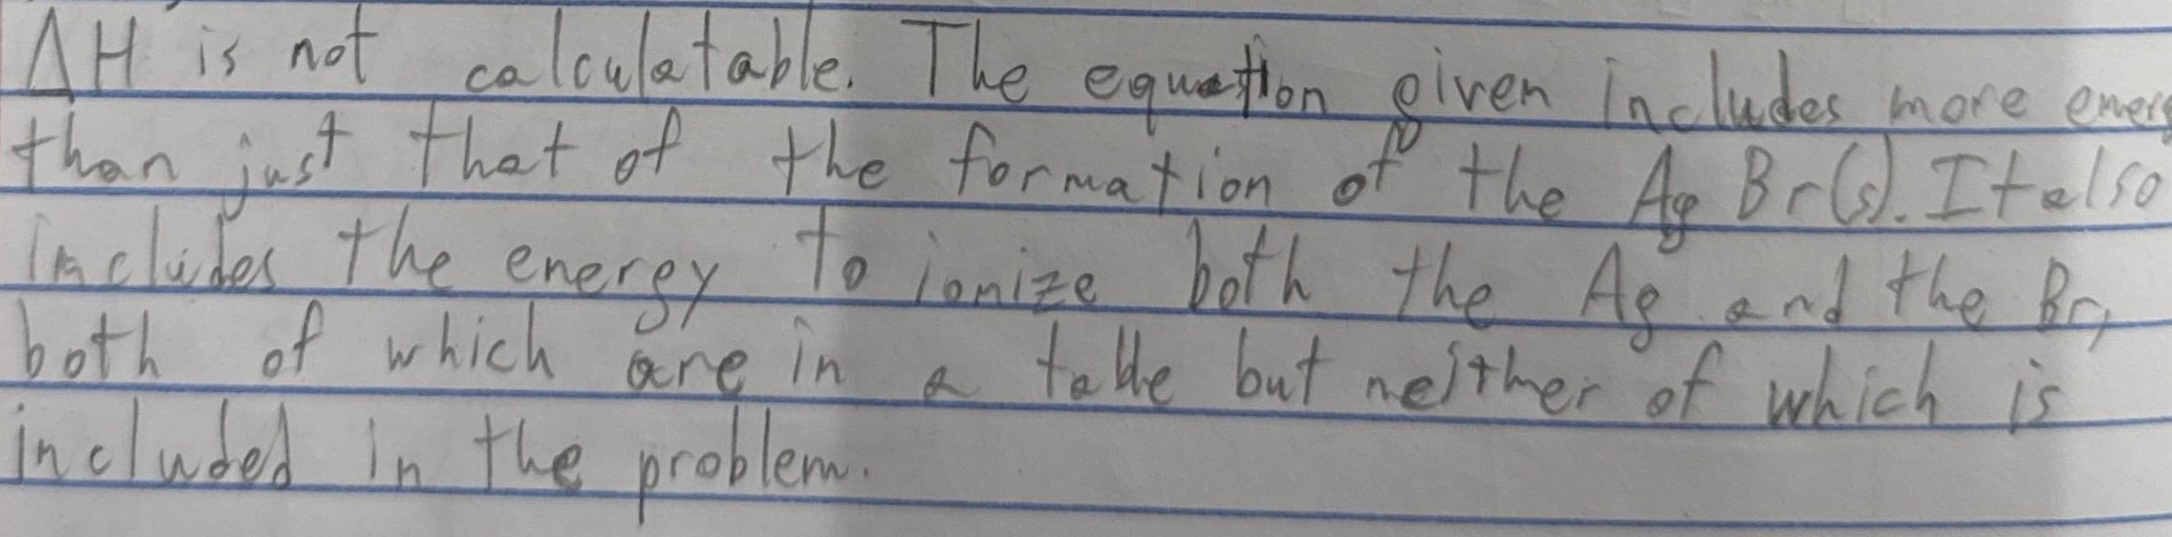
\includegraphics[width=\textwidth]{Answers Images/D29.jpg}
            \end{center}



    \pagebreak
    \section{Topic D Problem 30}
        Calculate the volume of gaseous \ce{C4H10} (butane) at 25.00\unit{\celsius} 
        and 785.0 torr that must be burned in a closed, rigid container if you want to obtain enough heat to convert 15.50 g of ice at 0.00\unit{\celsius} into steam at 100.00\unit{\celsius}. 
        Use the following information:\\
        $\rm \Delta H_f^{\circ}$ of \ce{C4H10(g)} = -149.1 kJ/mol\\
        $\rm \Delta H_f^{\circ}$ of \ce{H2O(l)} = -285.8 kJ/mol\\
        $\rm \Delta H_f^{\circ}$ of \ce{CO2(g)} = -393.5 kJ/mol\\
        $\rm \Delta H_{fusion}$ of ice = 6.009 kJ/mol\\
        $\rm \Delta H_{vaporization}$ of water = 40.67 kJ/mol at 100\unit{\celsius}\\
        Average specific heat capacity of liquid water in the range 0\unit{\celsius} to 100\unit{\celsius} = 4.174 \unit{\frac{\joule}{\gram\cdot\celsius}}.
        Do not look up any other thermochemical information. 

        \subsection{Solution}
            \begin{center}
                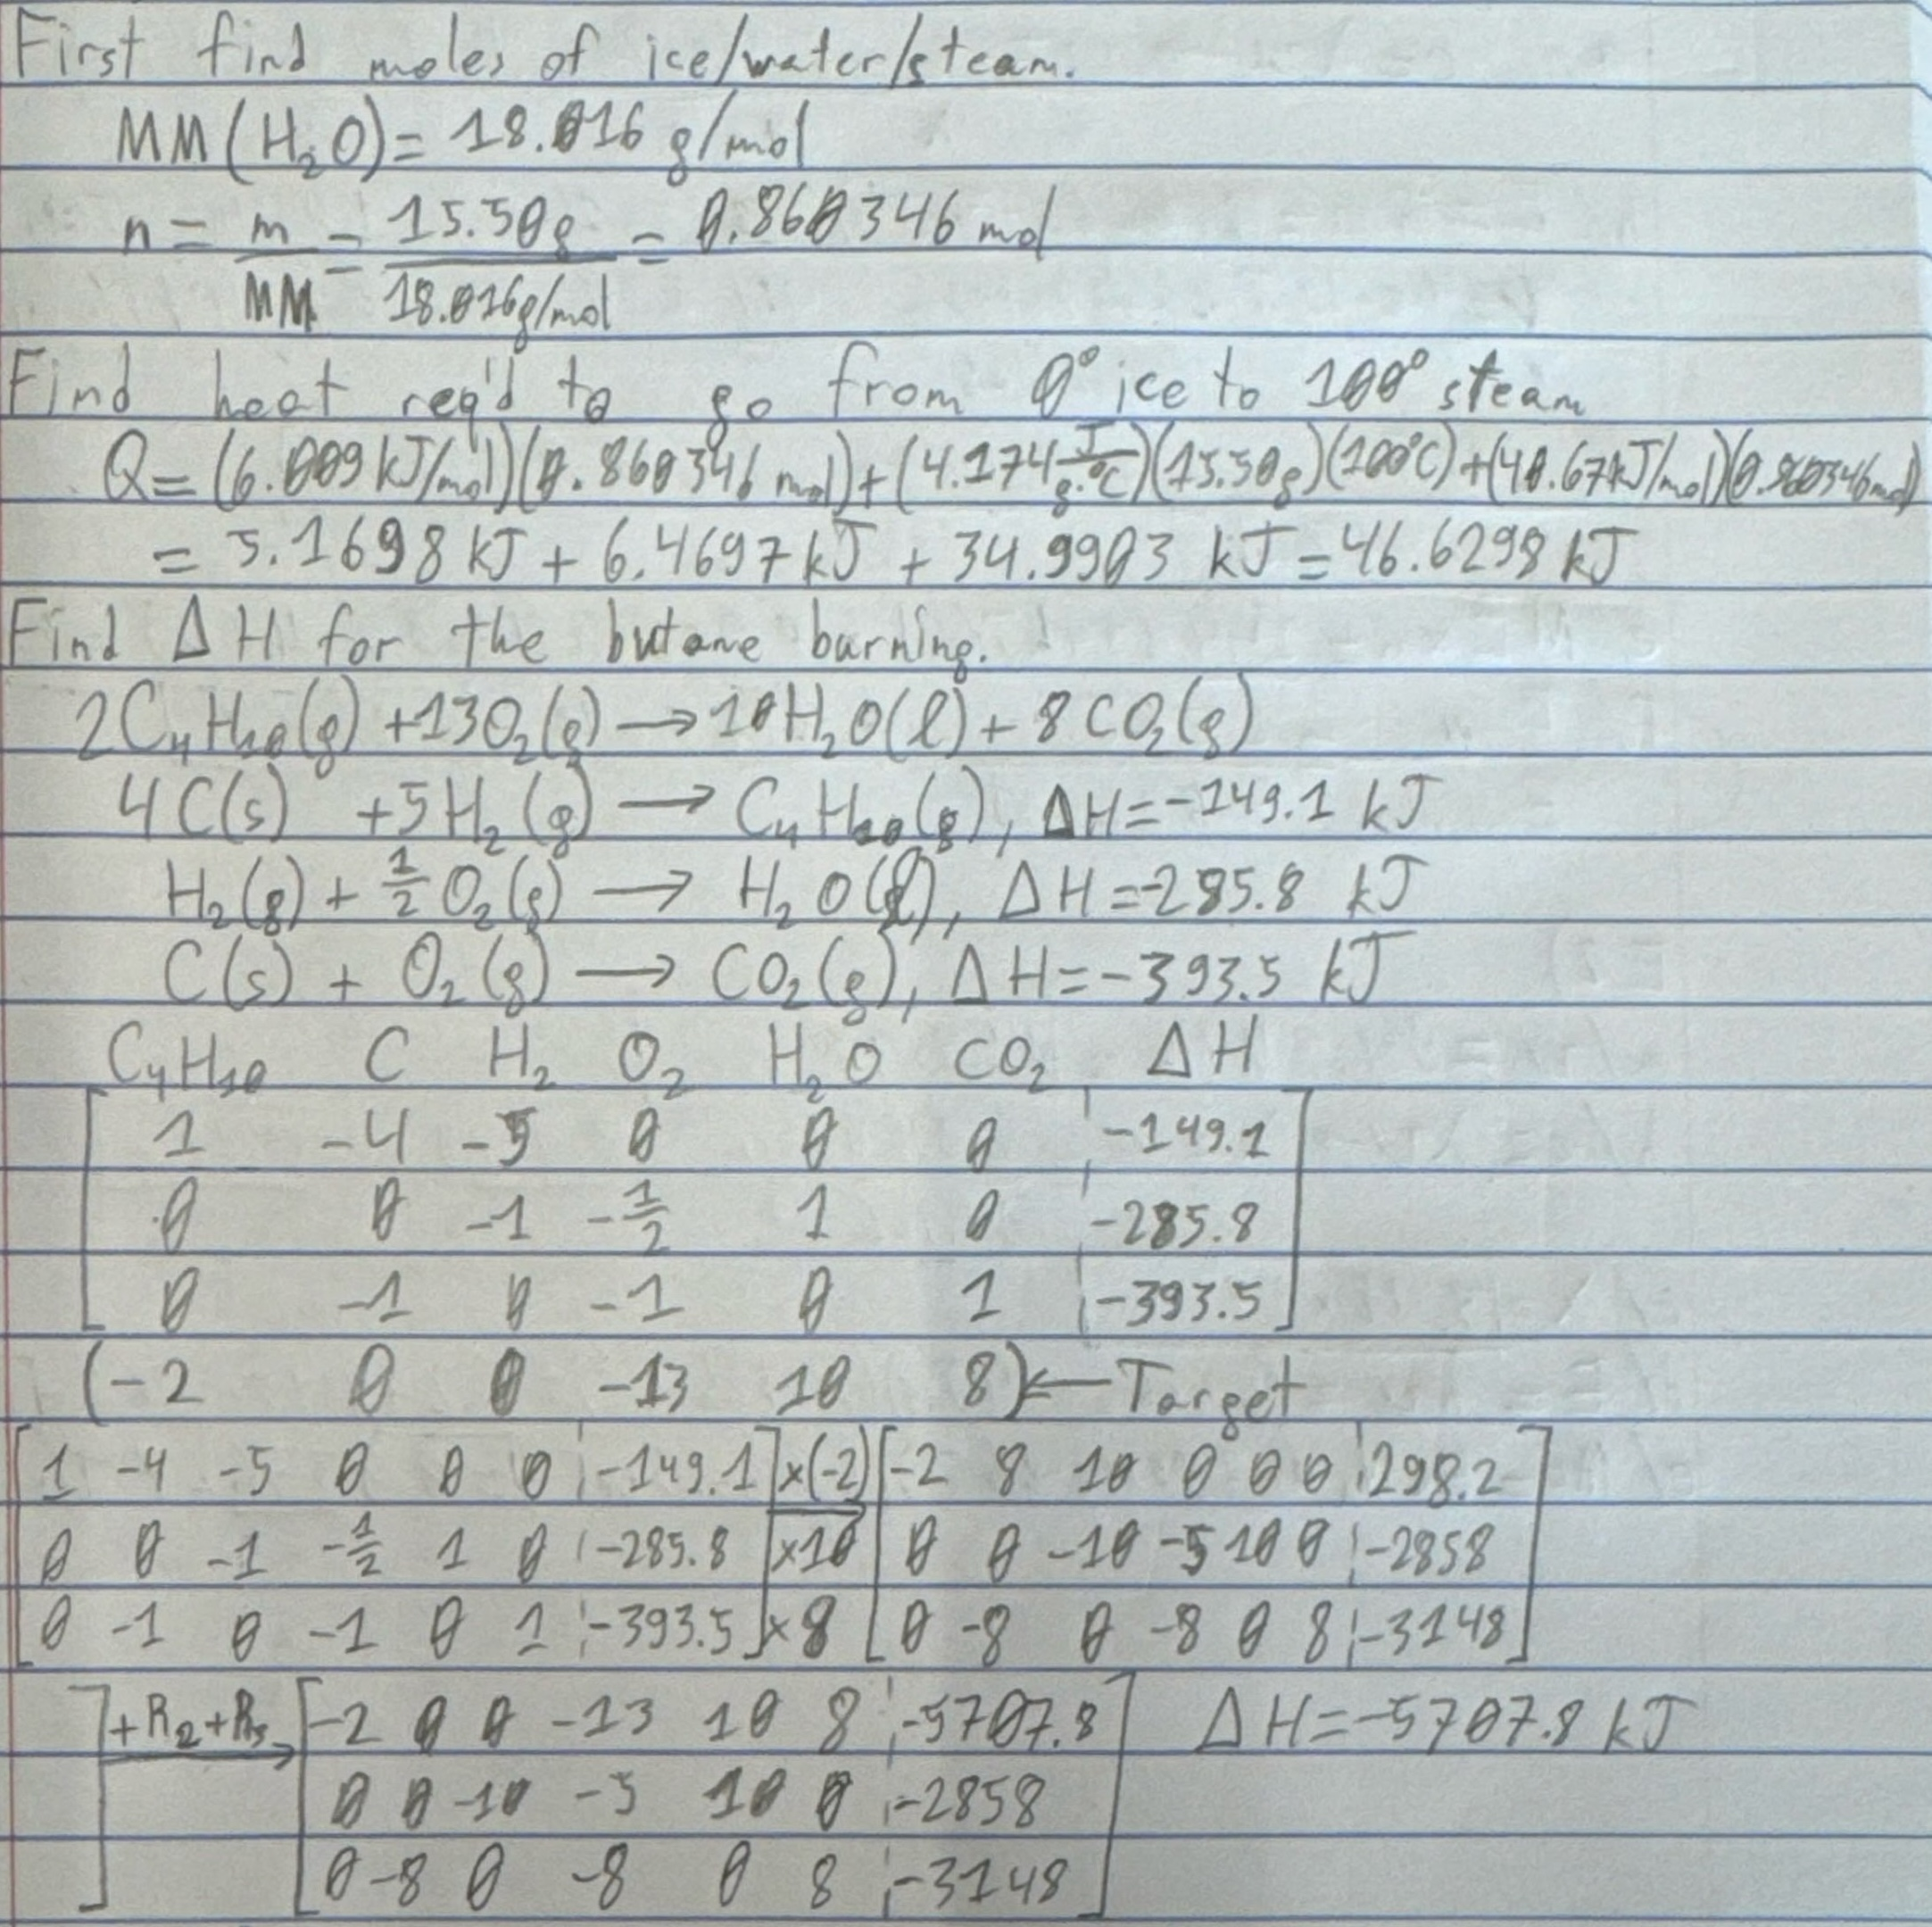
\includegraphics[width=\textwidth]{Answers Images/D30-1.jpg}
            \end{center}
            At this point, since the container is of constant volume, we use $\Delta$E, not $\rm\Delta H$, the former of which we should find now. 
            In our equation, we can see that $\rm \Delta n_{gas} = -7\,\unit{\mole}$. 
            \begin{align}
                \rm
                \Delta H    &=  \rm \Delta E + RT\,\Delta n_{gas}\\
                \Delta E    &=  \rm \Delta H - RT\,\Delta n_{gas}\\
                    &=  -5707.8\,\unit{\kilo\joule} - (8.314\,\unit{\frac{\joule}{\mole\,\kelvin}}) (298.15\unit{\kelvin}) (-7\,\unit{\mole})\\
                    &=  -5707.8\,\unit{\kilo\joule} + 17.4\,\unit{\kilo\joule}
                    =   -5690.4\,\unit{\kilo\joule}
            \end{align}

            From here, we use our favorite ratio.
            \begin{align}
                n_{\rm sp}  &=  \frac{n\,\Delta E_{\rm sp}}{\Delta E}
                    =   \frac{(2\,\unit{\mole}) \times (-\U{46.62}98\,\unit{\kilo\joule})}{-5690.4\,\unit{\kilo\joule}}
                    =   0.0\U{16388}8\,\unit{\mole}
            \end{align}

            Lastly, we use the Ideal Gas Law.
            \begin{align}
                PV  &=  nRT\\
                V   &=  \frac{n_{\rm sp} RT}{P}
                    =   \frac{(0.0\U{16388}8\,\unit{\mole})(62.36\,\unit{\frac{\torr\,\liter}{\mole\,\kelvin}})(298.15\unit{\kelvin})}{785.0\,\unit{\torr}}\\
                    &=  0.\U{3881}6675\,\unit{\liter}
                    =   \boxed{388.2\,\unit{\milli\liter}}
            \end{align}

    \setcounter{section}{0}
    \pagebreak
    \section{Topic E Problem 1}
        Calculate the following properties of light that has a wavelength of 490 nm.
        \begin{enumerate}[label=\alph*)]
            \item   The frequency
            \item   The energy of one photon, in joules
            \item   The photon energy in kJ/mol
            \item   The number of moles of photons required to supply 10.0 kJ of energy
            \item   The total energy of 0.0125 moles of photons
            \item   The number of individual photons required to supply 25.0 J of energy.
        \end{enumerate}

        \subsection{Solution}
            \begin{center}
                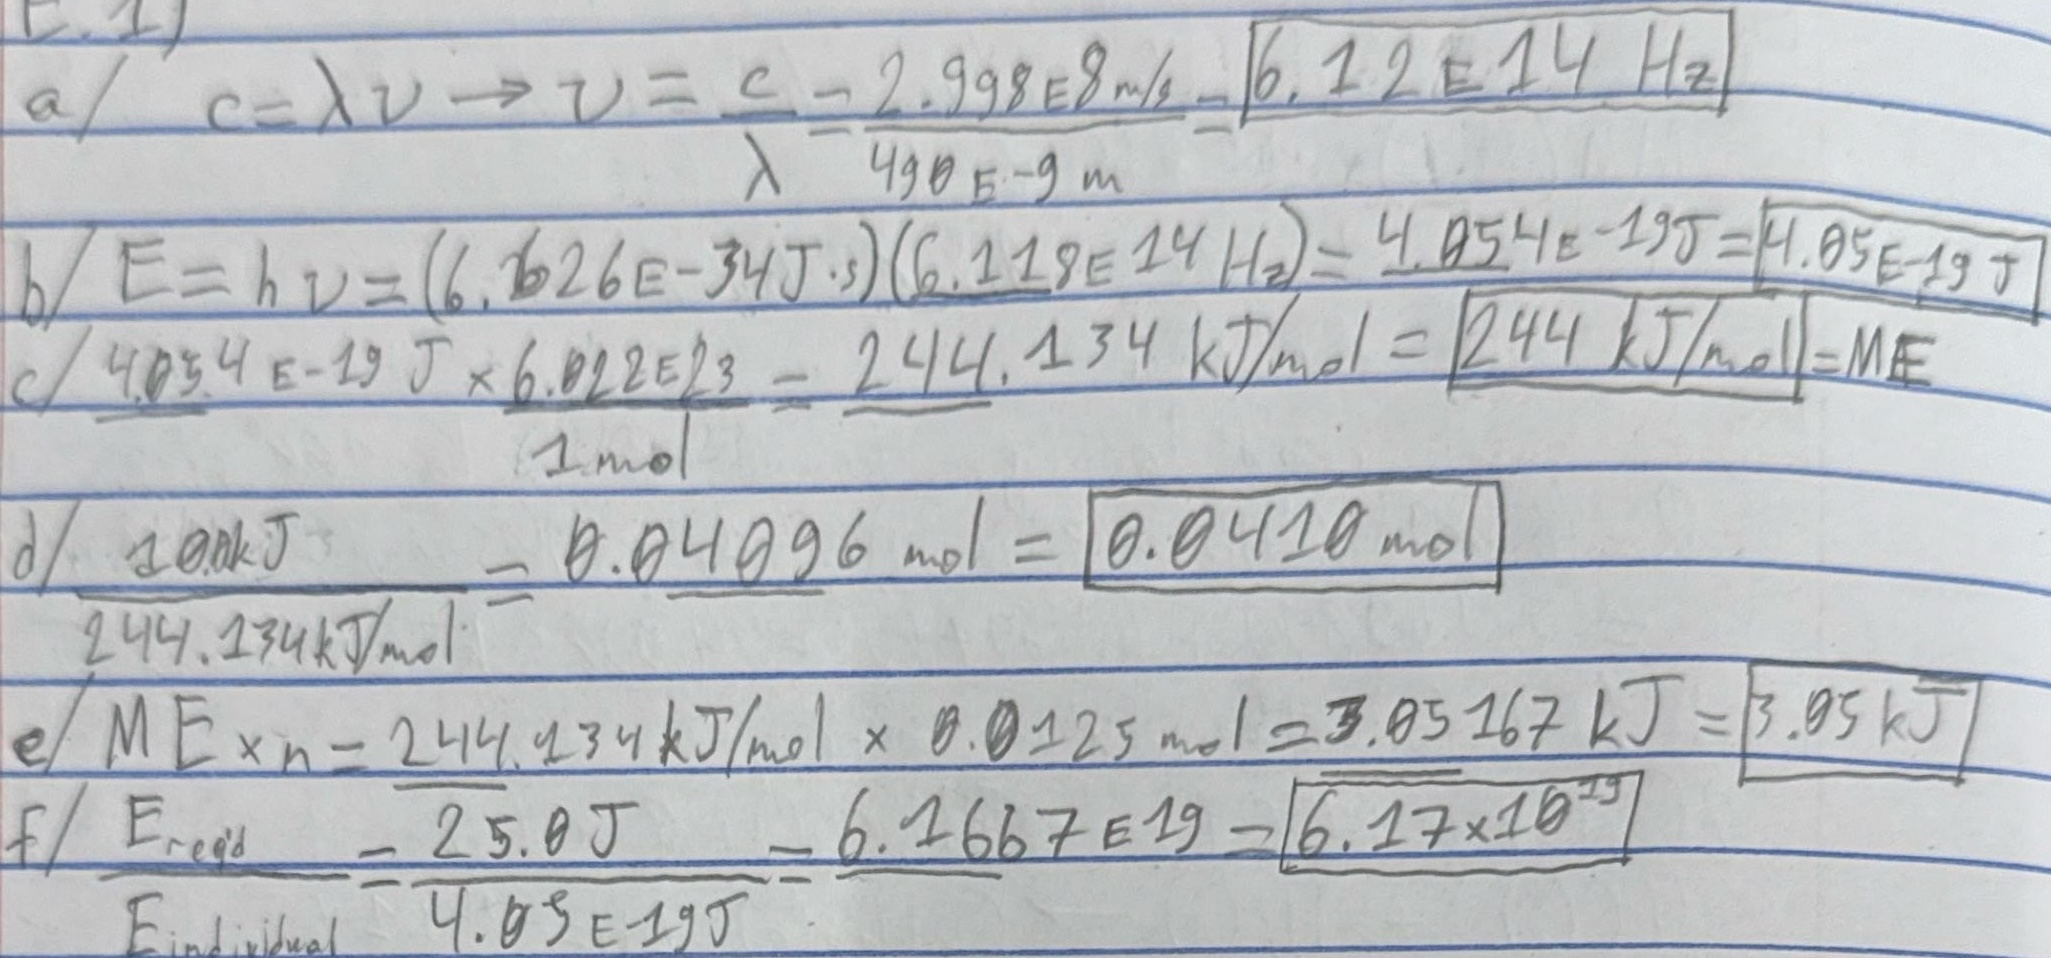
\includegraphics[width=\textwidth]{Answers Images/E1.jpg}
            \end{center}


    \pagebreak
    \section{Topic E Problem 2}
        Frequencies of FM radio stations are usually given in megahertz (MHz), where 1 MHz equals 106 sec$^{-1}$. 
        For a radio station that broadcasts at 94.3 MHz, calculate the following:
        \begin{enumerate}[label=\alph*)]
            \item   The frequency in sec$^{-1}$
            \item   The wavelength of the radiation, in meters
            \item   The wavelength of the radiation, in nanometers
            \item   The photon energy, in joules
            \item   The photon energy, in kJ/mol
        \end{enumerate}
        
        \subsection{Solution}
            \begin{center}
                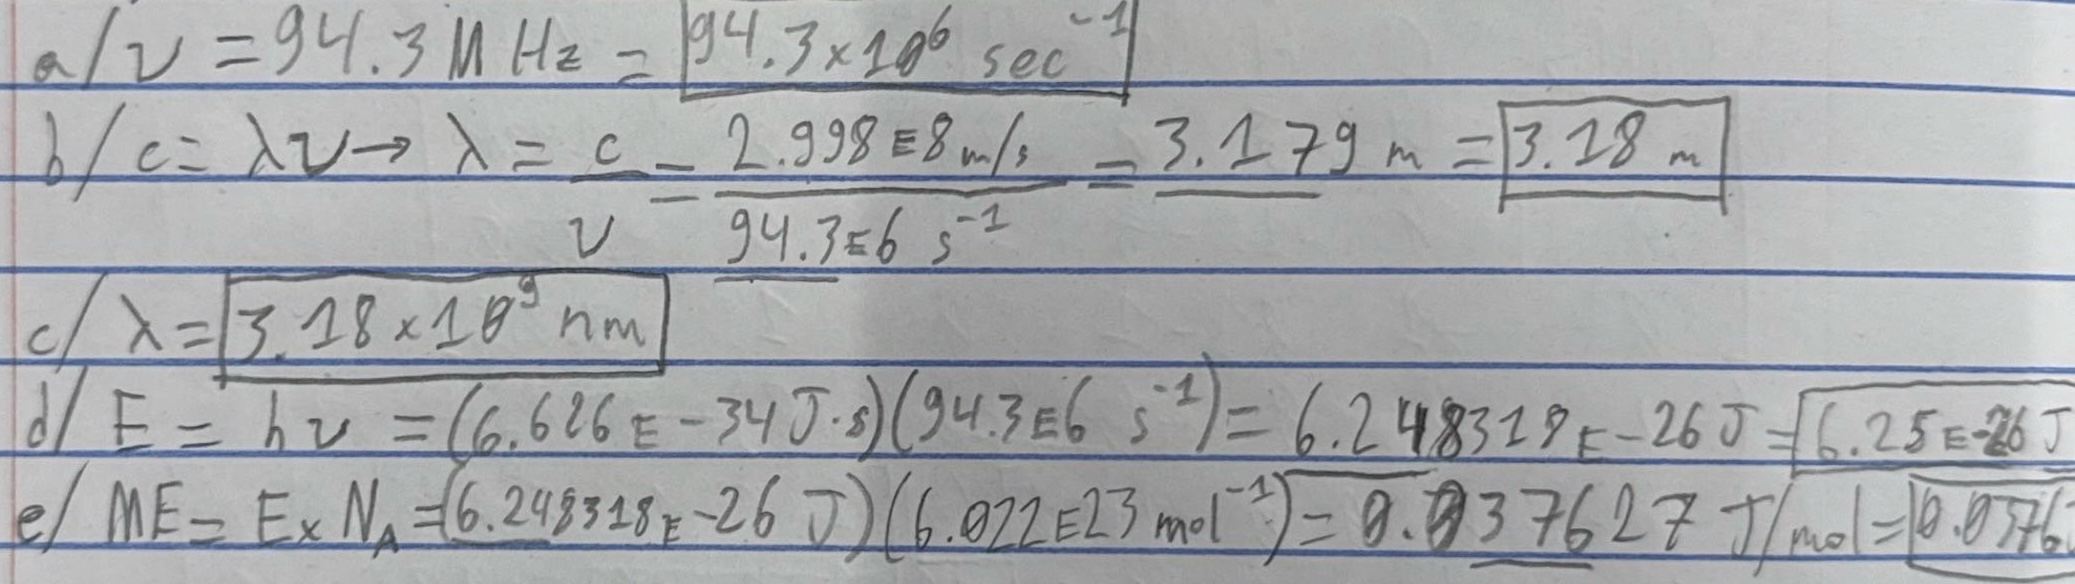
\includegraphics[width=\textwidth]{Answers Images/E2.jpg}
            \end{center}
            The answer to part (e) is 0.376\,\unit{\joule/\mole} if you have trouble reading it.


    \pagebreak
    \section{Topic E Problem 3}
        Molecular bromine (\ce{Br2}) breaks apart into bromine atoms if it is exposed to light whose energy is 190 kJ/mol.
        \begin{enumerate}[label=\alph*)]
            \item   Calculate the wavelength of this light, in nanometers.
            \item   Does this light fall in the visible spectrum? 
                If not, does it fall in the infrared region, or in the ultraviolet region?
        \end{enumerate}

        \subsection{Solution (a)}
            Here, $ME$ refers to the molar energy, meaning the amount of energy per mole.
            \begin{align}
                E   &=  \frac{ME}{N_A}
                    =   \frac{190\E{3}\,\unit{\kilo\joule/\mole}}{6.022\E{23}\,\unit{\mole^{-1}}}
                    =   \U{3.15}5\E{-19}\,\unit{\joule}\\
                E   &=  h\nu\\
                \nu &=  \frac{E}{h}
                    =   \frac{\U{3.15}5\E{-19}\,\unit{\joule}}{6.626\E{-34}\,\unit{\joule\cdot\second}}
                    =   \U{4.76}169\E{14}\,\unit{\hertz}\\
                \lambda &=  \frac{\rm c}{\nu}
                    =   \frac{2.998\E{8}\,\unit{\meter/\second}}{\U{4.76}169\E{14}\,\unit{\hertz}}
                    =   \U{6.29}60796\E{-7}\,\unit{\meter}\\
                    &=  \U{629}.60796\,\unit{\nano\meter}
                    =   \boxed{630\,\unit{\nano\meter}}
            \end{align}
        
        \subsection{Solution (b)}
            This \U{does} fall in the visible spectrum.
            The visible spectrum runs from about 400\,\unit{\nano\meter} to 700\,\unit{\nano\meter}.

    % \pagebreak
    \section{Topic E Problem 4}
        When an atom absorbs light, does an electron in the atom move from a lower energy level to a higher energy level, or does it move from a higher level to a lower level?

        \subsection{Solution}
        Absorbing causes it to move from a lower level to a higher level. 


    \pagebreak
    \section{Topic E Problem 5}
        Here are two of the allowed energy levels for a lithium atom:
        \begin{center}
            Level 2: $-8.638\E{-19}$ J; Level 3: $-5.678\E{-19}$ J
        \end{center}
        \begin{enumerate}[label=\alph*)]
            \item   What is $\Delta$E for a lithium atom when an electron moves from level 3 to level 2? 
                Give your answer in joules.
            \item   What is $\Delta$E for a lithium atom when an electron moves from level 2 to level 3? 
                Give your answer in joules.
            \item   Convert your answer to part a into kJ/mol.
            \item   When the electron drops from level 3 to level 2, the atom emits a photon. 
                Calculate the wavelength of this photon, in nanometers.
            \item   Can visible light move an electron from level 2 to level 3? 
                Explain your answer.
        \end{enumerate}

        \subsection{Solution (a)}
            \begin{align*}
                \Delta E    &=  E_2 - E_3
                    =   -8.638\E{-19}\,\unit{\joule} + 5.678\E{-19}\,\unit{\joule}
                    =   \boxed{-2.960\E{-19}\,\unit{\joule}}
            \end{align*}
        
        \subsection{Solution (b)}
            \begin{align*}
                \Delta E    &=  E_3 - E_2
                    =   -5.678\E{-19}\,\unit{\joule} + 8.638\E{-19}\,\unit{\joule}
                    =   \boxed{2.960\E{-19}\,\unit{\joule}}
            \end{align*}

        \subsection{Solution (c)}
            \begin{align}
                ME  &=  E \times N_A
                    =   -2.960\E{-19}\,\unit{\joule} \times 6.022\E{23}\,\unit{\mole^{-1}}\\
                    &=  -\U{17.82}512\E{4}\,\unit{\joule/\mole}
                    =   \boxed{-178.3\,\unit{\kilo\joule/\mole}}
            \end{align}

        \subsection{Solution (d)}
            The energy of the photon would be the negative of the energy lost when jumping from level 3 to level 2.
            \begin{gather}
                E   =   h\nu
                    =   \frac{hc}{\lambda}\\
                \begin{align}
                    \lambda &=  \frac{hc}{E}
                        =   \frac{(6.626\E{-34}\,\unit{\joule\cdot\second})(2.998\E{8}\,\unit{\meter/\second})}{2.960\E{-19}\,\unit{\joule}}\\
                        &=  6.711\E{-7}\,\unit{\meter}
                        =   \boxed{671.1\,\unit{\nano\meter}}
                \end{align}
            \end{gather}
        
        \subsection{Solution (e)}
            Visible light ranging from 400nm to 700nm, it could, so the answer is yes.
            It would be on the edge of the spectrum, though, so some people might not be able to see it.

    % \pagebreak
    \section{Topic E Problem 6}
        An atom can only undergo one electron transition at a time. 
        However, when we observe the emission spectrum of an element, we see many lines. 
        Explain.

        \subsection{Solution}
            When we observe the emission spectrum of an element, we are often observing the emission spectrum of many different atoms of that element and not just one.
            One atom may absorb the wavelength for one color, while another atom may absorb the wavelength for another color.
            The emission spectrum we see (such as on a spectrometer) is merely the total of all of these emitted colors.
            We can think of it less as a spectrum and more as a statistical graph of the total number of data points at specific values being represented by the presence and boldness of a spectrum line at that wavelength.

    \pagebreak
    \section{Topic E Problem 7}
        Here are three of the allowed energy levels for a calcium atom:
        \begin{center}
            Level A: -710.3 kJ/mol; Level B: -648.4 kJ/mol; Level C: -514.2 kJ/mol
        \end{center}
        Calculate the wavelengths of the three emission lines that can be produced by electron transitions involving these levels, and list the initial and final level for each emission line.

        \subsection{Solution A and B}
            Going from B to A would be the direction in which the electron lowers in energy and releases a photon.
            Wavelength is calculatable from energy, whch is itself calculatable from molar energy.
            \begin{gather}
                E   =   \frac{hc}{\lambda}; ME  =   E * N_A\\
                \begin{align}
                    \Delta ME   &=  ME_B - ME_A
                        =   -648.4\,\unit{\kilo\joule/\mole} + 710.3\,\unit{\kilo\joule/\mole}\\
                        &=  61.9\E{3}\,\unit{\joule/\mole}\\
                    \lambda &=  \frac{hc}{E}
                        =   \frac{hcN_A}{ME}\\
                        &=  \frac{(6.626\E{-34}\,\unit{\joule\cdot\second})(2.998\E{8}\,\unit{\meter/\second})(6.022\E{23}\,\unit{\mol^{-1}})}{61.9\E{3}\,\unit{\joule/\mole}}\\
                        &=  \frac{0.\U{1196}255\,\unit{\meter}}{61.9\E{3}}
                        =   \U{1.932}56\E{-6}\,\unit{\meter}
                        =   \boxed{1.933\E{-6}\,\unit{\meter}}
                \end{align}
            \end{gather}
        
        \subsection{Solution B and C}
            It would go from C to B to release a photon.
            \begin{align}
                \Delta ME   &=  ME_C - ME_B
                    =   -514.2\,\unit{\kilo\joule/\mole} + 648.4\,\unit{\kilo\joule/\mole}\\
                    &=  134.2\E{3}\,\unit{\joule/\mole}\\
                \lambda &=  \frac{hc}{E}
                    =   \frac{hcN_A}{ME}\\
                    &=  \frac{(6.626\E{-34}\,\unit{\joule\cdot\second})(2.998\E{8}\,\unit{\meter/\second})(6.022\E{23}\,\unit{\mol^{-1}})}{134.2\E{3}\,\unit{\joule/\mole}}\\
                    &=  \frac{0.\U{1196}255\,\unit{\meter}}{134.2\E{3}}
                    =   \U{8.913}97\E{-7}\,\unit{\meter}
                    =   \boxed{8.914\E{-7}\,\unit{\meter}}
            \end{align}
        
        \subsection{Solution A and C}
            It would go from C to A to release a photon.
            \begin{align}
                \Delta ME   &=  ME_C - ME_A
                    =   -514.2\,\unit{\kilo\joule/\mole} + 710.3\,\unit{\kilo\joule/\mole}\\
                    &=  196.1\E{3}\,\unit{\joule/\mole}\\
                \lambda &=  \frac{hc}{E}
                    =   \frac{hcN_A}{ME}\\
                    &=  \frac{(6.626\E{-34}\,\unit{\joule\cdot\second})(2.998\E{8}\,\unit{\meter/\second})(6.022\E{23}\,\unit{\mol^{-1}})}{196.1\E{3}\,\unit{\joule/\mole}}\\
                    &=  \frac{0.\U{1196}255\,\unit{\meter}}{196.1\E{3}}
                    =   \U{6.100}23\E{-7}\,\unit{\meter}
                    =   \boxed{6.100\E{-7}\,\unit{\meter}}
            \end{align}


    \pagebreak
    \section{Topic E Problem 8}
        A line in the emission spectrum of neon has a wavelength of 471.5 nm. 
        The final energy level for the corresponding electron transition is -266.7 kJ/mol. 
        What is the initial energy level for this transition?

        \subsection{Solution}
            The wavelength of the line correspond to the change in the energy from the initial to the final wavelength.
            Since this is an emission of light rather than an absorption, the change in energy will be have to be negative.
            \begin{align}
                \Delta ME   &=  -N_A * \frac{hc}{\lambda}\\
                    &=  -\frac{(6.626\E{-34}\,\unit{\joule\cdot\second})(2.998\E{8}\,\unit{\meter/\second})(6.022\E{23}\,\unit{\mol^{-1}})}{471.5\E{-9}\,\unit{\meter}}\\
                    &=  -\frac{0.\U{1196}255}{471.5\E{-9}}\,\unit{\joule/\mole}
                    =   -\U{253.7}126\,\unit{\kilo\joule/\mole}\\
                ME_i    &=  ME_f - \Delta ME
                    =   -266.7\,\unit{\kilo\joule/\mole} + \U{253.7}126\,\unit{\kilo\joule/\mole}\\
                    &=  -\U{13.0}126\,\unit{\kilo\joule/\mole}
                    =   \boxed{-13.0\,\unit{\kilo\joule/\mole}}
            \end{align}


    \pagebreak
    \section{Topic E Problem 9}
        The following electronic transitions and the corresponding wavelengths can be seen in the emission spectrum of potassium:
        \begin{center}
            \begin{tabular}{l l}
                level 7 $\rightarrow$ level 6   &wavelength = 770.1 nm\\
                level 8 $\rightarrow$ level 7   &wavelength = 1243.6 nm\\
                level 10 $\rightarrow$ level 8  &wavelength = 14,818.5 nm
            \end{tabular}
        \end{center}
        Using this information, calculate the wavelength that corresponds to the level 10 $\rightarrow$ level 6 transition in a potassium atom.

        \subsection{Solution}
            This is a four-step process. 
            Step one: convert wavelength to energy.
            I will keep Planck's constant and the speed of light as constants for the time being.
            \begin{gather}
                E_{7,6} =   \frac{hc}{770.1\,\unit{\nano\meter}}\\
                E_{8,7} =   \frac{hc}{1243.6\,\unit{\nano\meter}}\\
                E_{10,8}=   \frac{hc}{14818.5\,\unit{\nano\meter}}
            \end{gather}

            Step two: add the three energies together to get the energy required to go from level 10 to level 6.
            We can also pull out the $hc$ since it's a constant in all three.
            \begin{align}
                E_{10,6}    &=  E_{10,8} + E_{8,7} + E_{7,6}\\
                    &=  \frac{hc}{14818.5\,\unit{\nano\meter}} + \frac{hc}{1243.6\,\unit{\nano\meter}} + \frac{hc}{770.1\,\unit{\nano\meter}}\\
                    &=  hc\left( \frac{1}{14818.5\,\unit{\nano\meter}} + \frac{1}{1243.6\,\unit{\nano\meter}} + \frac{1}{770.1\,\unit{\nano\meter}} \right)
            \end{align}

            Step three: since $E = \frac{hc}{\lambda}$, we can divide both sides by $hc$ to find the reciprocal of the wavelength.
            \begin{equation}
                \frac{E_{10,6}}{hc} =   \frac{1}{\lambda_{10,6}}
                    =   \frac{1}{14818.5\,\unit{\nano\meter}} + \frac{1}{1243.6\,\unit{\nano\meter}} + \frac{1}{770.1\,\unit{\nano\meter}}
            \end{equation}

            Step four: Take the reciprocal to get the final answer.
            \begin{align}
                \lambda_{10,6}  &=  \left( \frac{1}{14818.5\,\unit{\nano\meter}} + \frac{1}{1243.6\,\unit{\nano\meter}} + \frac{1}{770.1\,\unit{\nano\meter}} \right)^{-1}
                    =   \boxed{460.8\,\unit{\nano\meter}}
            \end{align}

            For anyone interested in the more math-physics behind this, this does set up an equation for the equivalent wavelength for multiple emitted or absorbed wavelengths.
            \begin{equation}
                \lambda_{\rm eq}    =   \left( \sum \lambda_i^{-1} \right)^{-1}
            \end{equation}
    \pagebreak
    \tableofcontents
\end{document}